\documentclass[a4paper,12pt]{article}

\usepackage{graphicx}
\usepackage{hyperref}
\usepackage{amssymb}
\usepackage{amsmath}
\usepackage{karnaugh-map}

\title{Computation Organisation (CSE1400) --- Summary}
\author{Dany Sluijk}
\date{October 2018}

\makeindex
  
\begin{document}
\maketitle
\begin{center}
	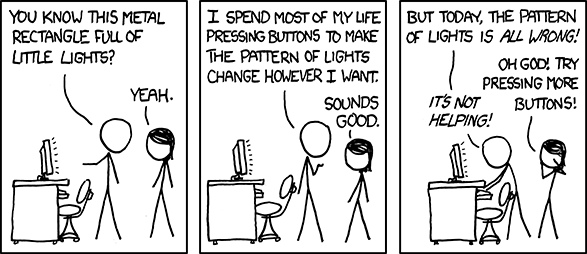
\includegraphics[height=5cm]{./intro}
\end{center}
\begin{abstract}
	This document contains a summary of the Computation Organisation course given
	in the first year of Computer Science and Engineering.
	This is \emph{not} a definitive guide, and might contain errors.
	Please send an email to \href{mailto:dany@atlasdev.nl}{``dany@atlasdev.nl''}.
	This summary is distributed under the
  \href{https://opensource.org/licenses/MIT}{MIT} license.
\end{abstract}

\newpage
\tableofcontents

\section{Number Representation}

By default the standard binary system can only represent unsigned integers.
With other number representation systems you can also represent signed numbers and floats.
This chapter describes different number systems.

\subsection{Sign \& Magnitude}
{\bf Sign \& Magnitude} is the (for humans) the simplest method of representing numbers.
You add one bit at the most significant bit (the `sign' bit).
This bit defines if the rest of the bitstring is positive or negative.
A \(0\) indicates a positive number, a \(1\) a negative one.
Applying direct operations to these numbers does not work, for example \(5 + -5\).
When you do this with Sign \& Magnitude you'll end up with \(2\).
This is obviously not correct.
Also you end up with two zero's, \(0000\) and \(1000\).

\begin{table}[h]
	\centering
	\begin{tabular}{c | c | c}
		Decimal & Binary    & S \& M    \\
		\hline
		72      & 0100 1000 & 0100 1000 \\
		-57     & --        & 1011 1001 \\
		8       & 0000 1000 & 0000 1000 \\
		-8      & --        & 1000 1000 \\
		-43.75  & --        & --        \\
	\end{tabular}
	\caption{Sign \& Magnitude}
\end{table}

\subsection{One's Complement}
{\bf One's complement} is the same as Sign \& Magnitude,
but when the sign is positive you need to take the complement of the number.
It's a lot better for computer to work with, but you still cannot directly do operations to it.
If you do attempt to do calculations to it, you will get an offset of \(1\).

\begin{table}[h]
	\centering
	\begin{tabular}{c | c | c}
		Decimal & Binary    & One's Complement \\
		\hline
		72      & 0100 1000 & 0100 1000        \\
		-57     & --        & 1100 0110        \\
		8       & 0000 1000 & 0000 1000        \\
		-8      & --        & 1111 0111        \\
		-43.75  & --        & --               \\
	\end{tabular}
	\caption{One's Complement}
\end{table}

\subsection{Two's Complement}
{\bf Two's complement} is the same as one's complement.
The difference is that you'll add 1 to the result when the number is negative.
This also makes sure there is only one zero.

\begin{table}[h]
	\centering
	\begin{tabular}{c | c | c}
		Decimal & Binary    & Two's Complement \\
		\hline
		72      & 0100 1000 & 0100 1000        \\
		-57     & --        & 1100 0111        \\
		8       & 0000 1000 & 0000 1000        \\
		-8      & --        & 1111 1000        \\
		-43.75  & --        & --               \\
	\end{tabular}
	\caption{Two's Complement}
\end{table}

\subsection{Excess-N}
{\bf Excess-N} is great for really large positive or negative numbers.
The \(N\) in Excess-N stands for the offset used.
For example, if you want to represent \(5\) you can do \(5 + N\).
This gives \(5 + 3 = 8\) in Excess-3.
To get the \(5\) back you can just substract the \(N\) to the number.
For example \(8 - 3 = 5\).

\begin{table}[h]
	\centering
	\begin{tabular}{c | c | c | c}
		Decimal & Binary    & Excess-128 & Excess-57 \\
		\hline
		72      & 0100 1000 & 1100 1000  & 1000 0001 \\
		-57     & --        & 0100 0111  & 0000 0000 \\
		8       & 0000 1000 & 1000 1000  & 0100 0001 \\
		-8      & --        & 0111 1000  & 0011 0001 \\
		-43.75  & --        & --         & --        \\
	\end{tabular}
	\caption{Excess-N}
\end{table}

\subsection{IEEE-754}
{\bf IEEE-754} is an way of representing floats.
It has the following parts:

\begin{table}[h]
	\centering
	\begin{tabular}{l | c | c| l}
		Name     & Bits (32-bit) & Bits (64-bit) & Description                    \\
		\hline
		Sign     & 1             & 1             & 0 for positive, 1 for negative \\
		Exponent & 8             & 11            & Exponent for the Mantissa      \\
		Mantissa & 23            & 52            & The actual number, encodeds    \\
	\end{tabular}
	\caption{Parts of IEEE-754}
\end{table}

To convert a number to IEEE-754 you first have to convert the number to binary.
Let's take the number \(-43.75\).
We can already see that the sign bit should be 1, as the number is negative.
Let's first convert the interger first part, this gives \(0010 1011\).
Then convert the decimal part seperately and add it.
This gives \(0010 1011 . 1100\).
Now move the point to the first \(1\) and remember the places you've moved.
This gives \(001.0 1011 1100\), with 5 places moved.
The 5 is your exponent, but it needs a bias to deal with negative numbers.
With 32-bit the bias is \(127\), in 64-bit \(1023\).
We are using 32-bit, so apply a bias of \(127\).
This gives an exponent of \(exp = 5 + 127 = 132\) or \(1000 0100\).
For the mantissa part you copy all digits after the dot and right-pad with 0's till 23 bits.
This gives you \(010 1111 0000 0000 0000 0000\).
The complete format IEEE-754 gives \(1100 0010 0010 1111 0000 0000 0000 0000\)

\begin{table}[h]
	\centering
	\begin{tabular}{c | c | c | c | c}
		Decimal & Binary    & Sign & Exponent  & Mantissa                     \\
		\hline
		72      & 0100 1000 & 0    & 1000 0101 & 001 0000 0000 0000 0000 0000 \\
		-57     & --        & 1    & 1000 0100 & 110 0100 0000 0000 0000 0000 \\
		8       & 0000 1000 & 0    & 1000 0010 & 000 0000 0000 0000 0000 0000 \\
		-8      & --        & 1    & 1000 0010 & 000 0000 0000 0000 0000 0000 \\
		-43.75  & --        & 1    & 1000 0100 & 010 1111 0000 0000 0000 0000 \\
	\end{tabular}
	\caption{IEEE-754}
\end{table}


\end{document}